\chapter{Test}
\section{A}
\begin{itemize}
	\item Verteidigung: 15-20min präsi, 30min diskussion
\end{itemize}
	





\chapter{Combining Stuff}
\section{Notation MM as Sentential tokens}
\section{Notation MM as graphical editor base}
\section{Conclude graphical editor integrated in the grammar at Symbol, Seq, or Alt positions}
\section{what misses? Text <-> Model sync}





\subsection{Introduction}
Requirements:
\begin{itemize}
	\item In contrast to Xtexts node model which is just updated during parsing and used to guide unparsing, the Notation metamodel must be equivalent to a valid token stream and therefore describe it unambigiously. 
	\item It must contain or refer to all information to nesessary to create a specific token stream together with a language model and a grammar model.   
	\item it has to be a parsetree in order to create language elements if the correspoding tokens exist.
	\item it should offer GMF stuff elements \todo{add what GMF has interesting}
	explicit, seperated from language model
\end{itemize}




\section{old ==>}
%	-------------- Latex testing --------------
The Notation model is an EMF model to describe a tree. A node or leaf contains a reference to the describing language model element.The notation model bridges the token stream and the abstract syntax. It is the parse tree, and thus also describes a valid concrete syntax representation of the model.  It is a mandatory to updated or created it when generating a concrete representation of the model. If the notation model (element) was created to complement a language model (element), the notation model (element) serves as a disambiguis bulding plan to create the token stream for a valid concrete representation. In gereral, the notation model saves information which is not stored in the language model but relevant for presentation. It also keeps a generic, type save reference on the represented language object.\\
Each notation element represents (part of) a language element and should be a stable container for different visual representations of that element with addionaly layout information.  Due to this, if an element has multiple semantically equivalent representations, it is possible to switch the representation without switching the notation element. A switch would invalidade the descendants of the current node. A notion element therefore contains a transient structural feature containing all possible valid concrete representation rules, the non-transient last representation rule and optional the last user selected representation rule. In case these representation rules are grammar rules, they must be complemented with addionional information in order to make the token production unambigious. For example a grammar rule like:
\begin{xtxt}
A : (B | C) "myKeyword"
\end{xtxt}
would be translated to the following productions rules 
\begin{xtxt}
A - > B "myKeyword"
A - > C "myKeyword"
\end{xtxt}
for the sake of abstraction and simplicity, this distinction, especially im more complex scenarios, should be hidden from the language developer. In a case where B and C are semantically equivalent  it is arbitrary from the abstract syntax perspective if an A contains a B or C. The notation element must close this gap, so an notation element refering to a lanuage element represented by A doesn't need to store the keyword "myKeyword", this information is implicit, but it must distinguish if the concrete presentation of this particular A should use B or C as a presentation selection. It is therefore not nessecary to explicity assign  a production rule but to implicity make one resolvable by dissolving the ambiguity for options and choices which have no representation in the language model. \\
The base class for representation rules must be general, or unspecific, enough allow non textual representations. Notation elements should prefer containment references instead of attributes to easy to ease merging, like the GMF notation model. In contrast to GMF, this driving motivation is not team support but easier automatic updating between old and new versions.\\
In order to integrate with incremental parsing, notation model elements should hold a transient integer which contains the distance to the first previous token accesing the current one in it's lookahead. \\
Finally, a notation model element should contain a flag if it is currently textually visible.
\todo{ rewrites possible}
\todo{ reason that a representation in text editor is necessary}
\todo{mention that addtionaly layout information can be added to a node}





%\begin{figure}
%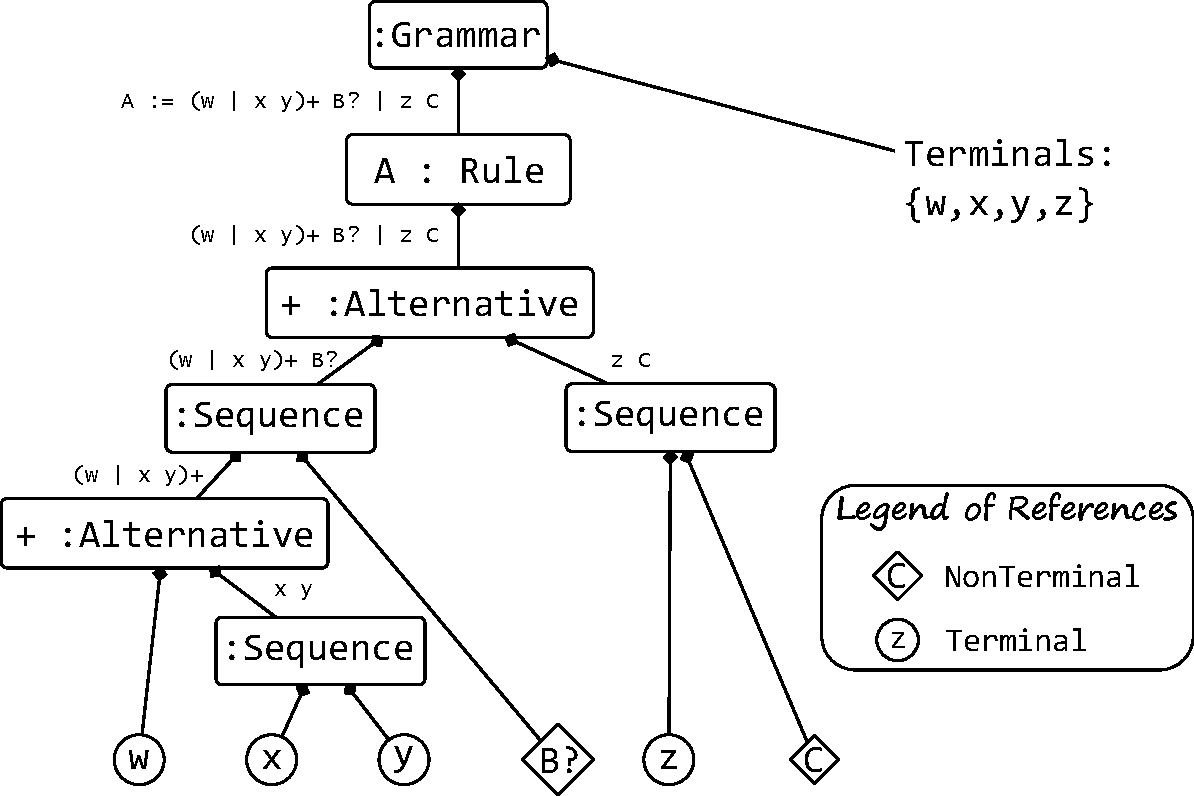
\includegraphics[scale=0.7]{gfx/ex/grammarExample} 
%\caption{Example Rule ``A := (w |x y)+ B? | z C''}
%\end{figure}
%\FloatBarrier
 

%\begin{figure}
%% %\import{gfx/svgExport/}{grammarExample.eps_tex}
%  \centering
%  
\includegraphics[scale=1.00]{gfx/temp/fhw} 
%  \caption{Schematic data flow for a web application}
%  \label{fig:architecture:web_app_usage}
%\end{figure}
